\documentclass[]{article}
\usepackage{lmodern}
\usepackage{amssymb,amsmath}
\usepackage{ifxetex,ifluatex}
\usepackage{fixltx2e} % provides \textsubscript
\ifnum 0\ifxetex 1\fi\ifluatex 1\fi=0 % if pdftex
  \usepackage[T1]{fontenc}
  \usepackage[utf8]{inputenc}
\else % if luatex or xelatex
  \ifxetex
    \usepackage{mathspec}
  \else
    \usepackage{fontspec}
  \fi
  \defaultfontfeatures{Ligatures=TeX,Scale=MatchLowercase}
\fi
% use upquote if available, for straight quotes in verbatim environments
\IfFileExists{upquote.sty}{\usepackage{upquote}}{}
% use microtype if available
\IfFileExists{microtype.sty}{%
\usepackage{microtype}
\UseMicrotypeSet[protrusion]{basicmath} % disable protrusion for tt fonts
}{}
\usepackage[margin=1in]{geometry}
\usepackage{hyperref}
\hypersetup{unicode=true,
            pdftitle={HW1: Predictive Analytics},
            pdfauthor={Faizan Khalid Mohsin},
            pdfborder={0 0 0},
            breaklinks=true}
\urlstyle{same}  % don't use monospace font for urls
\usepackage{color}
\usepackage{fancyvrb}
\newcommand{\VerbBar}{|}
\newcommand{\VERB}{\Verb[commandchars=\\\{\}]}
\DefineVerbatimEnvironment{Highlighting}{Verbatim}{commandchars=\\\{\}}
% Add ',fontsize=\small' for more characters per line
\usepackage{framed}
\definecolor{shadecolor}{RGB}{248,248,248}
\newenvironment{Shaded}{\begin{snugshade}}{\end{snugshade}}
\newcommand{\KeywordTok}[1]{\textcolor[rgb]{0.13,0.29,0.53}{\textbf{#1}}}
\newcommand{\DataTypeTok}[1]{\textcolor[rgb]{0.13,0.29,0.53}{#1}}
\newcommand{\DecValTok}[1]{\textcolor[rgb]{0.00,0.00,0.81}{#1}}
\newcommand{\BaseNTok}[1]{\textcolor[rgb]{0.00,0.00,0.81}{#1}}
\newcommand{\FloatTok}[1]{\textcolor[rgb]{0.00,0.00,0.81}{#1}}
\newcommand{\ConstantTok}[1]{\textcolor[rgb]{0.00,0.00,0.00}{#1}}
\newcommand{\CharTok}[1]{\textcolor[rgb]{0.31,0.60,0.02}{#1}}
\newcommand{\SpecialCharTok}[1]{\textcolor[rgb]{0.00,0.00,0.00}{#1}}
\newcommand{\StringTok}[1]{\textcolor[rgb]{0.31,0.60,0.02}{#1}}
\newcommand{\VerbatimStringTok}[1]{\textcolor[rgb]{0.31,0.60,0.02}{#1}}
\newcommand{\SpecialStringTok}[1]{\textcolor[rgb]{0.31,0.60,0.02}{#1}}
\newcommand{\ImportTok}[1]{#1}
\newcommand{\CommentTok}[1]{\textcolor[rgb]{0.56,0.35,0.01}{\textit{#1}}}
\newcommand{\DocumentationTok}[1]{\textcolor[rgb]{0.56,0.35,0.01}{\textbf{\textit{#1}}}}
\newcommand{\AnnotationTok}[1]{\textcolor[rgb]{0.56,0.35,0.01}{\textbf{\textit{#1}}}}
\newcommand{\CommentVarTok}[1]{\textcolor[rgb]{0.56,0.35,0.01}{\textbf{\textit{#1}}}}
\newcommand{\OtherTok}[1]{\textcolor[rgb]{0.56,0.35,0.01}{#1}}
\newcommand{\FunctionTok}[1]{\textcolor[rgb]{0.00,0.00,0.00}{#1}}
\newcommand{\VariableTok}[1]{\textcolor[rgb]{0.00,0.00,0.00}{#1}}
\newcommand{\ControlFlowTok}[1]{\textcolor[rgb]{0.13,0.29,0.53}{\textbf{#1}}}
\newcommand{\OperatorTok}[1]{\textcolor[rgb]{0.81,0.36,0.00}{\textbf{#1}}}
\newcommand{\BuiltInTok}[1]{#1}
\newcommand{\ExtensionTok}[1]{#1}
\newcommand{\PreprocessorTok}[1]{\textcolor[rgb]{0.56,0.35,0.01}{\textit{#1}}}
\newcommand{\AttributeTok}[1]{\textcolor[rgb]{0.77,0.63,0.00}{#1}}
\newcommand{\RegionMarkerTok}[1]{#1}
\newcommand{\InformationTok}[1]{\textcolor[rgb]{0.56,0.35,0.01}{\textbf{\textit{#1}}}}
\newcommand{\WarningTok}[1]{\textcolor[rgb]{0.56,0.35,0.01}{\textbf{\textit{#1}}}}
\newcommand{\AlertTok}[1]{\textcolor[rgb]{0.94,0.16,0.16}{#1}}
\newcommand{\ErrorTok}[1]{\textcolor[rgb]{0.64,0.00,0.00}{\textbf{#1}}}
\newcommand{\NormalTok}[1]{#1}
\usepackage{graphicx,grffile}
\makeatletter
\def\maxwidth{\ifdim\Gin@nat@width>\linewidth\linewidth\else\Gin@nat@width\fi}
\def\maxheight{\ifdim\Gin@nat@height>\textheight\textheight\else\Gin@nat@height\fi}
\makeatother
% Scale images if necessary, so that they will not overflow the page
% margins by default, and it is still possible to overwrite the defaults
% using explicit options in \includegraphics[width, height, ...]{}
\setkeys{Gin}{width=\maxwidth,height=\maxheight,keepaspectratio}
\IfFileExists{parskip.sty}{%
\usepackage{parskip}
}{% else
\setlength{\parindent}{0pt}
\setlength{\parskip}{6pt plus 2pt minus 1pt}
}
\setlength{\emergencystretch}{3em}  % prevent overfull lines
\providecommand{\tightlist}{%
  \setlength{\itemsep}{0pt}\setlength{\parskip}{0pt}}
\setcounter{secnumdepth}{0}
% Redefines (sub)paragraphs to behave more like sections
\ifx\paragraph\undefined\else
\let\oldparagraph\paragraph
\renewcommand{\paragraph}[1]{\oldparagraph{#1}\mbox{}}
\fi
\ifx\subparagraph\undefined\else
\let\oldsubparagraph\subparagraph
\renewcommand{\subparagraph}[1]{\oldsubparagraph{#1}\mbox{}}
\fi

%%% Use protect on footnotes to avoid problems with footnotes in titles
\let\rmarkdownfootnote\footnote%
\def\footnote{\protect\rmarkdownfootnote}

%%% Change title format to be more compact
\usepackage{titling}

% Create subtitle command for use in maketitle
\providecommand{\subtitle}[1]{
  \posttitle{
    \begin{center}\large#1\end{center}
    }
}

\setlength{\droptitle}{-2em}

  \title{HW1: Predictive Analytics}
    \pretitle{\vspace{\droptitle}\centering\huge}
  \posttitle{\par}
    \author{Faizan Khalid Mohsin}
    \preauthor{\centering\large\emph}
  \postauthor{\par}
      \predate{\centering\large\emph}
  \postdate{\par}
    \date{May 14, 2019}

\usepackage{booktabs}
\usepackage{longtable}
\usepackage{array}
\usepackage{multirow}
\usepackage{wrapfig}
\usepackage{float}
\usepackage{colortbl}
\usepackage{pdflscape}
\usepackage{tabu}
\usepackage{threeparttable}
\usepackage{threeparttablex}
\usepackage[normalem]{ulem}
\usepackage{makecell}
\usepackage{xcolor}

\begin{document}
\maketitle

\begin{Shaded}
\begin{Highlighting}[]
\KeywordTok{rm}\NormalTok{(}\DataTypeTok{list=}\KeywordTok{ls}\NormalTok{())}

\NormalTok{knitr}\OperatorTok{::}\NormalTok{opts_chunk}\OperatorTok{$}\KeywordTok{set}\NormalTok{(}\DataTypeTok{echo =} \OtherTok{TRUE}\NormalTok{)}

\KeywordTok{source}\NormalTok{(}\StringTok{'a1_functions_train.r'}\NormalTok{)}
\KeywordTok{load}\NormalTok{(}\StringTok{'a1_simulated_data.RData'}\NormalTok{)}

\CommentTok{#library(installr)}
\CommentTok{#updateR() }

\CommentTok{#Load all packages}
\KeywordTok{library}\NormalTok{(missForest)}
\end{Highlighting}
\end{Shaded}

\begin{verbatim}
## Loading required package: randomForest
\end{verbatim}

\begin{verbatim}
## randomForest 4.6-14
\end{verbatim}

\begin{verbatim}
## Type rfNews() to see new features/changes/bug fixes.
\end{verbatim}

\begin{verbatim}
## Loading required package: foreach
\end{verbatim}

\begin{verbatim}
## Loading required package: itertools
\end{verbatim}

\begin{verbatim}
## Loading required package: iterators
\end{verbatim}

\begin{Shaded}
\begin{Highlighting}[]
\KeywordTok{require}\NormalTok{(kableExtra)}
\end{Highlighting}
\end{Shaded}

\begin{verbatim}
## Loading required package: kableExtra
\end{verbatim}

\begin{Shaded}
\begin{Highlighting}[]
\KeywordTok{require}\NormalTok{(tableone)}
\end{Highlighting}
\end{Shaded}

\begin{verbatim}
## Loading required package: tableone
\end{verbatim}

\begin{Shaded}
\begin{Highlighting}[]
\KeywordTok{require}\NormalTok{(ggplot2)}
\end{Highlighting}
\end{Shaded}

\begin{verbatim}
## Loading required package: ggplot2
\end{verbatim}

\begin{verbatim}
## Registered S3 methods overwritten by 'ggplot2':
##   method         from 
##   [.quosures     rlang
##   c.quosures     rlang
##   print.quosures rlang
\end{verbatim}

\begin{verbatim}
## 
## Attaching package: 'ggplot2'
\end{verbatim}

\begin{verbatim}
## The following object is masked from 'package:randomForest':
## 
##     margin
\end{verbatim}

\begin{Shaded}
\begin{Highlighting}[]
\KeywordTok{require}\NormalTok{(UsingR)}
\end{Highlighting}
\end{Shaded}

\begin{verbatim}
## Loading required package: UsingR
\end{verbatim}

\begin{verbatim}
## Loading required package: MASS
\end{verbatim}

\begin{verbatim}
## Loading required package: HistData
\end{verbatim}

\begin{verbatim}
## Loading required package: Hmisc
\end{verbatim}

\begin{verbatim}
## Loading required package: lattice
\end{verbatim}

\begin{verbatim}
## Loading required package: survival
\end{verbatim}

\begin{verbatim}
## Loading required package: Formula
\end{verbatim}

\begin{verbatim}
## 
## Attaching package: 'Hmisc'
\end{verbatim}

\begin{verbatim}
## The following objects are masked from 'package:base':
## 
##     format.pval, units
\end{verbatim}

\begin{verbatim}
## 
## Attaching package: 'UsingR'
\end{verbatim}

\begin{verbatim}
## The following object is masked from 'package:survival':
## 
##     cancer
\end{verbatim}

\begin{Shaded}
\begin{Highlighting}[]
\KeywordTok{require}\NormalTok{(glmnet)}
\end{Highlighting}
\end{Shaded}

\begin{verbatim}
## Loading required package: glmnet
\end{verbatim}

\begin{verbatim}
## Loading required package: Matrix
\end{verbatim}

\begin{verbatim}
## Loaded glmnet 2.0-16
\end{verbatim}

\begin{Shaded}
\begin{Highlighting}[]
\KeywordTok{require}\NormalTok{(knitr)}
\end{Highlighting}
\end{Shaded}

\begin{verbatim}
## Loading required package: knitr
\end{verbatim}

\begin{Shaded}
\begin{Highlighting}[]
\KeywordTok{require}\NormalTok{(dplyr)}
\end{Highlighting}
\end{Shaded}

\begin{verbatim}
## Loading required package: dplyr
\end{verbatim}

\begin{verbatim}
## 
## Attaching package: 'dplyr'
\end{verbatim}

\begin{verbatim}
## The following objects are masked from 'package:Hmisc':
## 
##     src, summarize
\end{verbatim}

\begin{verbatim}
## The following object is masked from 'package:MASS':
## 
##     select
\end{verbatim}

\begin{verbatim}
## The following object is masked from 'package:kableExtra':
## 
##     group_rows
\end{verbatim}

\begin{verbatim}
## The following object is masked from 'package:randomForest':
## 
##     combine
\end{verbatim}

\begin{verbatim}
## The following objects are masked from 'package:stats':
## 
##     filter, lag
\end{verbatim}

\begin{verbatim}
## The following objects are masked from 'package:base':
## 
##     intersect, setdiff, setequal, union
\end{verbatim}

\begin{Shaded}
\begin{Highlighting}[]
\KeywordTok{require}\NormalTok{(epiR)}
\end{Highlighting}
\end{Shaded}

\begin{verbatim}
## Loading required package: epiR
\end{verbatim}

\begin{verbatim}
## Package epiR 0.9-99 is loaded
\end{verbatim}

\begin{verbatim}
## Type help(epi.about) for summary information
\end{verbatim}

\begin{verbatim}
## 
\end{verbatim}

\begin{Shaded}
\begin{Highlighting}[]
\KeywordTok{require}\NormalTok{(class)}
\end{Highlighting}
\end{Shaded}

\begin{verbatim}
## Loading required package: class
\end{verbatim}

\begin{Shaded}
\begin{Highlighting}[]
\KeywordTok{library}\NormalTok{(rpart)}
\KeywordTok{library}\NormalTok{(tree)}
\KeywordTok{library}\NormalTok{(pROC)}
\end{Highlighting}
\end{Shaded}

\begin{verbatim}
## Type 'citation("pROC")' for a citation.
\end{verbatim}

\begin{verbatim}
## 
## Attaching package: 'pROC'
\end{verbatim}

\begin{verbatim}
## The following object is masked from 'package:glmnet':
## 
##     auc
\end{verbatim}

\begin{verbatim}
## The following objects are masked from 'package:stats':
## 
##     cov, smooth, var
\end{verbatim}

\begin{Shaded}
\begin{Highlighting}[]
\KeywordTok{library}\NormalTok{(mice)}
\end{Highlighting}
\end{Shaded}

\begin{verbatim}
## 
## Attaching package: 'mice'
\end{verbatim}

\begin{verbatim}
## The following objects are masked from 'package:base':
## 
##     cbind, rbind
\end{verbatim}

\begin{Shaded}
\begin{Highlighting}[]
\KeywordTok{library}\NormalTok{(ISLR)}
\KeywordTok{library}\NormalTok{(gplots)}
\end{Highlighting}
\end{Shaded}

\begin{verbatim}
## 
## Attaching package: 'gplots'
\end{verbatim}

\begin{verbatim}
## The following object is masked from 'package:stats':
## 
##     lowess
\end{verbatim}

\begin{Shaded}
\begin{Highlighting}[]
\KeywordTok{library}\NormalTok{(xtable)}
\end{Highlighting}
\end{Shaded}

\begin{verbatim}
## 
## Attaching package: 'xtable'
\end{verbatim}

\begin{verbatim}
## The following objects are masked from 'package:Hmisc':
## 
##     label, label<-
\end{verbatim}

\begin{Shaded}
\begin{Highlighting}[]
\KeywordTok{library}\NormalTok{(cluster)}
\KeywordTok{library}\NormalTok{(corrplot)}
\end{Highlighting}
\end{Shaded}

\begin{verbatim}
## corrplot 0.84 loaded
\end{verbatim}

\begin{Shaded}
\begin{Highlighting}[]
\KeywordTok{library}\NormalTok{(doParallel)}
\end{Highlighting}
\end{Shaded}

\begin{verbatim}
## Loading required package: parallel
\end{verbatim}

\begin{Shaded}
\begin{Highlighting}[]
\CommentTok{#library(doMC)}
\KeywordTok{library}\NormalTok{(tools)}
\end{Highlighting}
\end{Shaded}

\subsection{Helper Functions}\label{helper-functions}

\begin{Shaded}
\begin{Highlighting}[]
\NormalTok{check.dim <-}\StringTok{ }\ControlFlowTok{function}\NormalTok{(data) \{}
    \ControlFlowTok{if}\NormalTok{ (}\KeywordTok{is.na}\NormalTok{(}\KeywordTok{dim}\NormalTok{(data)[}\DecValTok{1}\NormalTok{])) \{}
\NormalTok{        data <-}\StringTok{ }\KeywordTok{matrix}\NormalTok{(data, }\KeywordTok{length}\NormalTok{(data), }\DecValTok{1}\NormalTok{)}
\NormalTok{    \}}
    \KeywordTok{return}\NormalTok{(data)}
\NormalTok{\}}

\CommentTok{#impute using the mean (assuming it's all numeric)}
\NormalTok{mean.imp <-}\StringTok{ }\ControlFlowTok{function}\NormalTok{(data) \{ }
\NormalTok{    data <-}\StringTok{ }\KeywordTok{check.dim}\NormalTok{(data)}
    \CommentTok{#stop('Complete this function.')}
    \CommentTok{#lapply(data, )}
    \ControlFlowTok{for}\NormalTok{ (i }\ControlFlowTok{in} \DecValTok{1}\OperatorTok{:}\KeywordTok{ncol}\NormalTok{(data))\{ }
\NormalTok{      data[}\KeywordTok{is.na}\NormalTok{(data[,i]),i] =}\StringTok{ }\KeywordTok{mean}\NormalTok{(data[,i], }\DataTypeTok{na.rm=}\OtherTok{TRUE}\NormalTok{)}
\NormalTok{    \}}
    \CommentTok{#for each variable in data, impute the missing values using the mean of the available values}
    \KeywordTok{return}\NormalTok{(data)}
\NormalTok{\}}

\CommentTok{#add missingness to a matrix or dataframe}
\NormalTok{miss.set.df <-}\StringTok{ }\ControlFlowTok{function}\NormalTok{(dat, prop, }\DataTypeTok{type.miss=}\StringTok{'mcar'}\NormalTok{) \{}
\NormalTok{    dat <-}\StringTok{ }\KeywordTok{check.dim}\NormalTok{(dat)}
    \ControlFlowTok{for}\NormalTok{ (i }\ControlFlowTok{in} \DecValTok{1}\OperatorTok{:}\KeywordTok{dim}\NormalTok{(dat)[}\DecValTok{2}\NormalTok{]) \{}
\NormalTok{        dat[,i] <-}\StringTok{ }\KeywordTok{miss.set.vec}\NormalTok{(dat[,i], prop, type.miss)}
\NormalTok{    \}}
    \KeywordTok{return}\NormalTok{(dat)}
\NormalTok{\}}
\CommentTok{# what is this ?miss.set.vec}

\CommentTok{#add misingness to a vector; mcar = at random; mnar = not at random (remove higher values)}
\NormalTok{miss.set.vec <-}\StringTok{ }\ControlFlowTok{function}\NormalTok{(x, prop, }\DataTypeTok{type.miss=}\StringTok{'mcar'}\NormalTok{) \{}
\NormalTok{    n.miss <-}\StringTok{ }\KeywordTok{rbinom}\NormalTok{(}\DecValTok{1}\NormalTok{, }\KeywordTok{length}\NormalTok{(x), prop)}
    \ControlFlowTok{if}\NormalTok{ (type.miss }\OperatorTok{==}\StringTok{ 'mcar'}\NormalTok{) \{}
\NormalTok{        miss.idx <-}\StringTok{ }\KeywordTok{sample}\NormalTok{(}\DecValTok{1}\OperatorTok{:}\KeywordTok{length}\NormalTok{(x), n.miss, }\DataTypeTok{replace=}\NormalTok{F)}
\NormalTok{    \} }\ControlFlowTok{else} \ControlFlowTok{if}\NormalTok{ (type.miss }\OperatorTok{==}\StringTok{ 'mnar'}\NormalTok{) \{}
\NormalTok{        miss.idx <-}\StringTok{ }\KeywordTok{order}\NormalTok{(x, }\DataTypeTok{decreasing=}\NormalTok{T)[}\DecValTok{1}\OperatorTok{:}\NormalTok{n.miss]}
\NormalTok{    \}}
\NormalTok{    x[miss.idx] <-}\StringTok{ }\OtherTok{NA}
    \KeywordTok{return}\NormalTok{(x)}
\NormalTok{\}}

\NormalTok{split.data <-}\StringTok{ }\ControlFlowTok{function}\NormalTok{(data, train.prop, }\DataTypeTok{set.seed=}\OtherTok{NA}\NormalTok{) \{}
    \ControlFlowTok{if}\NormalTok{ (}\OperatorTok{!}\KeywordTok{is.na}\NormalTok{(set.seed)) \{}\KeywordTok{set.seed}\NormalTok{(set.seed)\}}
\NormalTok{    train.idx <-}\StringTok{ }\KeywordTok{sample}\NormalTok{(}\DecValTok{1}\OperatorTok{:}\KeywordTok{dim}\NormalTok{(data)[}\DecValTok{1}\NormalTok{], }\KeywordTok{round}\NormalTok{(}\KeywordTok{dim}\NormalTok{(data)[}\DecValTok{1}\NormalTok{]}\OperatorTok{*}\NormalTok{train.prop), }\DataTypeTok{replace=}\NormalTok{F)}
\NormalTok{    test.idx <-}\StringTok{ }\KeywordTok{setdiff}\NormalTok{(}\DecValTok{1}\OperatorTok{:}\KeywordTok{dim}\NormalTok{(data)[}\DecValTok{1}\NormalTok{], train.idx)}
\NormalTok{    train.set <-}\StringTok{ }\NormalTok{data[train.idx,]}
\NormalTok{    test.set <-}\StringTok{ }\NormalTok{data[test.idx,]}
    \KeywordTok{return}\NormalTok{(}\KeywordTok{list}\NormalTok{(}\DataTypeTok{train=}\NormalTok{train.set, }\DataTypeTok{test=}\NormalTok{test.set))}
\NormalTok{\}}


\NormalTok{get.resid.err <-}\StringTok{ }\ControlFlowTok{function}\NormalTok{(train.set, test.set) \{}
    \CommentTok{#Train the models and get the MSE}
    \CommentTok{#stop('Complete this function.')}
  
    \CommentTok{#fit a linear model on the training set (train.set) using only the intercept Y ~ 1}
\NormalTok{  model1 =}\StringTok{ }\KeywordTok{lm}\NormalTok{(Y }\OperatorTok{~}\DecValTok{1}\NormalTok{, }\DataTypeTok{data =}\NormalTok{  train.set)}
  
    \CommentTok{#fit a linear model on the training set using all covariates Y ~ .}
\NormalTok{  modelfull =}\StringTok{ }\KeywordTok{lm}\NormalTok{(Y }\OperatorTok{~}\NormalTok{., train.set) }
  
    \CommentTok{#predict from each model on the test set (test.set)}
\NormalTok{  predict1 =}\StringTok{ }\KeywordTok{predict}\NormalTok{(model1, }\DataTypeTok{newdata =}\NormalTok{ test.set[,}\OperatorTok{-}\DecValTok{91}\NormalTok{])}
\NormalTok{  predict.full =}\StringTok{ }\KeywordTok{predict}\NormalTok{(modelfull, }\DataTypeTok{newdata =}\NormalTok{ test.set[,}\OperatorTok{-}\DecValTok{91}\NormalTok{])}
  
    \CommentTok{#calculate the mse of the null model}
\NormalTok{  mse.null =}\StringTok{ }\KeywordTok{mean}\NormalTok{((predict1 }\OperatorTok{-}\StringTok{ }\NormalTok{test.set}\OperatorTok{$}\NormalTok{Y)}\OperatorTok{^}\DecValTok{2}\NormalTok{)}
  
    \CommentTok{#calculate the mse of the full model}
\NormalTok{  mse.full =}\StringTok{ }\KeywordTok{mean}\NormalTok{((predict.full }\OperatorTok{-}\StringTok{ }\NormalTok{test.set}\OperatorTok{$}\NormalTok{Y)}\OperatorTok{^}\DecValTok{2}\NormalTok{)}
  
    \CommentTok{#calculate the residual error of the ratio of the latter over the former}
\NormalTok{    pred.res <-}\StringTok{ }\NormalTok{mse.full}\OperatorTok{/}\StringTok{ }\NormalTok{mse.null}
  
    \KeywordTok{return}\NormalTok{(pred.res)}
\NormalTok{\}}



\CommentTok{# Function to run the three imputations. }

\NormalTok{missing_function =}\StringTok{ }\ControlFlowTok{function}\NormalTok{(miss_type_idx, miss_prop_idx, data_idx)\{}
  
\NormalTok{  train.prop <-}\StringTok{ }\FloatTok{0.50}
\NormalTok{  train.split.seed <-}\StringTok{ }\DecValTok{78901}
\NormalTok{  outcome.var <-}\StringTok{ "Y"}
\NormalTok{  rf.iter <-}\StringTok{ }\DecValTok{12}
\NormalTok{  mice.iter <-}\StringTok{ }\DecValTok{10}
  
\NormalTok{  miss.prop.list <-}\StringTok{ }\KeywordTok{c}\NormalTok{(}\FloatTok{0.10}\NormalTok{, }\FloatTok{0.20}\NormalTok{, }\FloatTok{0.30}\NormalTok{, }\FloatTok{0.40}\NormalTok{) }\CommentTok{#proportion of missingness to assign}
\NormalTok{  miss.type.list <-}\StringTok{ }\KeywordTok{c}\NormalTok{(}\StringTok{'mcar'}\NormalTok{, }\StringTok{'mnar'}\NormalTok{) }\CommentTok{#mcar = missing completely at random; mnar = missing not at random}
\NormalTok{  data.idx <-}\StringTok{ }\NormalTok{data_idx }\CommentTok{#the dataset to use}
\NormalTok{  miss.type.idx <-}\StringTok{ }\NormalTok{miss_type_idx }\CommentTok{#type of missingness to use}
\NormalTok{  miss.prop.idx <-}\StringTok{ }\NormalTok{miss_prop_idx }\CommentTok{#proportio of missingness to use}
  
\NormalTok{  t.st <-}\StringTok{ }\KeywordTok{Sys.time}\NormalTok{() }\CommentTok{#time the run}
  
\NormalTok{  data <-}\StringTok{ }\NormalTok{data.list[[data.idx]]}
\NormalTok{  miss.prop <-}\StringTok{ }\NormalTok{miss.prop.list[miss.prop.idx]}
\NormalTok{  miss.type <-}\StringTok{ }\NormalTok{miss.type.list[miss.type.idx]}
  
\NormalTok{  split <-}\StringTok{ }\KeywordTok{split.data}\NormalTok{(data, train.prop, }\DataTypeTok{set.seed=}\NormalTok{train.split.seed)}
\NormalTok{  train.set <-}\StringTok{ }\NormalTok{split}\OperatorTok{$}\NormalTok{train; test.set <-}\StringTok{ }\NormalTok{split}\OperatorTok{$}\NormalTok{test}
\NormalTok{  pred.var <-}\StringTok{ }\KeywordTok{colnames}\NormalTok{(data)[}\OperatorTok{-}\KeywordTok{which}\NormalTok{(}\KeywordTok{colnames}\NormalTok{(data) }\OperatorTok{==}\StringTok{ }\NormalTok{outcome.var)]}
  
\NormalTok{  ##########################}
\NormalTok{  ## Set the missing data ##}
\NormalTok{  train.set.miss <-}\StringTok{ }\NormalTok{train.set}
\NormalTok{  train.set.miss[,pred.var] <-}\StringTok{ }\KeywordTok{miss.set.df}\NormalTok{(train.set.miss[,pred.var], miss.prop, miss.type)}
  
  \KeywordTok{dim}\NormalTok{(train.set.miss)}
  \KeywordTok{length}\NormalTok{(pred.var)}
  
\NormalTok{  ################}
  \CommentTok{#MICE Imputation}
\NormalTok{  mice.data <-}\StringTok{ }\NormalTok{train.set.miss}
  \KeywordTok{dim}\NormalTok{(mice.data)}
  
\NormalTok{  mice.data0 =}\StringTok{ }\NormalTok{mice.data[,pred.var]}
\NormalTok{  tempdata =}\StringTok{ }\KeywordTok{mice}\NormalTok{(mice.data0,}\DataTypeTok{m=}\NormalTok{mice.iter,}\DataTypeTok{maxit=}\DecValTok{25}\NormalTok{,}\DataTypeTok{meth=}\StringTok{'pmm'}\NormalTok{,}\DataTypeTok{seed=}\NormalTok{train.split.seed)}
  
  \CommentTok{# Will take the exptectation of the imputated data sets to obtain one data set. }
\NormalTok{  imputed =}\StringTok{ }\KeywordTok{complete}\NormalTok{(tempdata, }\DecValTok{1}\NormalTok{)}
  \ControlFlowTok{for}\NormalTok{ (i }\ControlFlowTok{in} \DecValTok{2}\OperatorTok{:}\NormalTok{mice.iter)\{}
    \KeywordTok{print}\NormalTok{(i)}
    \KeywordTok{print}\NormalTok{(}\KeywordTok{dim}\NormalTok{(imputed))}
\NormalTok{    imputed =}\StringTok{ }\NormalTok{imputed }\OperatorTok{+}\StringTok{ }\KeywordTok{complete}\NormalTok{(tempdata, i) }
    \KeywordTok{print}\NormalTok{(}\KeywordTok{dim}\NormalTok{(imputed))}
\NormalTok{  \}}
  
\NormalTok{  imputed =}\StringTok{ }\NormalTok{imputed }\OperatorTok{/}\StringTok{ }\NormalTok{mice.iter}
  
  
  \CommentTok{#run an imputation on the mice.data dataframe using the mice function from the mice package}
  \CommentTok{#use 'mice.iter' datasets and cap the iterations at 25}
  \CommentTok{#DO NOT INCLUDE the outcome 'Y' in the imputation, impute only mice.data[,pred.var]}
  \CommentTok{#try to parallelize the computation by running several interations in parallel}
  
\NormalTok{  mice.data.comp =}\StringTok{ }\KeywordTok{data.frame}\NormalTok{(imputed, }\DataTypeTok{Y =}\NormalTok{ mice.data}\OperatorTok{$}\NormalTok{Y)}
  \CommentTok{#write.csv(mice.data.comp, "mice_data_comp.csv", row.names = FALSE)}
  \CommentTok{#mice.data.comp = read.csv("mice_data_comp.csv")}
  \CommentTok{# same, but now as list, mild object}
  \CommentTok{# dslist <- complete(tempdata, "all")}
  \CommentTok{# length(dslist)}
  \CommentTok{# imputed_list_data = mean(dslist)}
  
  \CommentTok{# use package miceadds to save the imputed datasets. }
  \CommentTok{# require(miceadds)}
  \CommentTok{# write.mice.imputation(mi.res=tempdata, "tempdata1", include.varnames=TRUE,}
  \CommentTok{#       long=TRUE, mids2spss=TRUE, spss.dec=",", dattype=NULL)}
  
  \CommentTok{# # Parallalize mice imputation. }
  \CommentTok{# total.cores <- detectCores()}
  \CommentTok{# tempdata_core = parlmice(mice.data0, m = mice.iter, seed = NA, cluster.seed = 500, }
  \CommentTok{#                          n.core = total.cores,  n.imp.core = NULL, cl.type = "PSOCK")}
\NormalTok{  mice.data =}\StringTok{ }\NormalTok{mice.data.comp}
\NormalTok{  t.mice =}\StringTok{ }\KeywordTok{Sys.time}\NormalTok{() }\OperatorTok{-}\StringTok{ }\NormalTok{t.st}
  
  
\NormalTok{  t.st.mean =}\StringTok{ }\KeywordTok{Sys.time}\NormalTok{()}
\NormalTok{  #####################}
  \CommentTok{#Impute with the mean}
\NormalTok{  mean.data <-}\StringTok{ }\NormalTok{train.set.miss}
  
  \CommentTok{#finish the mean.imp function from the functions file and impute mean.data[,pred.var] }
  \CommentTok{# maybe should only use this mean.data[,pred.var] }
  
  \KeywordTok{head}\NormalTok{(}\KeywordTok{is.na}\NormalTok{(mean.data))}
  \KeywordTok{is.na}\NormalTok{(}\KeywordTok{dim}\NormalTok{(mean.data)[}\DecValTok{1}\NormalTok{])}
  \KeywordTok{check.dim}\NormalTok{(mean.data)}
  
  \CommentTok{# RUN the mean.imp function. }
\NormalTok{  mean.data =}\StringTok{ }\KeywordTok{mean.imp}\NormalTok{(mean.data)}
  \KeywordTok{all}\NormalTok{(}\OperatorTok{!}\KeywordTok{is.na}\NormalTok{(mean.data))}
  
  \CommentTok{# Testing if the mean.imp() function works. }
  \KeywordTok{all}\NormalTok{(}\KeywordTok{sapply}\NormalTok{(train.set.miss, }\ControlFlowTok{function}\NormalTok{(x) }\KeywordTok{mean}\NormalTok{(x, }\DataTypeTok{na.rm  =}\NormalTok{ T)) }\OperatorTok{==}\StringTok{ }\KeywordTok{sapply}\NormalTok{(mean.data, mean))}
  \KeywordTok{summary}\NormalTok{(}\KeywordTok{sapply}\NormalTok{(train.set.miss, }\ControlFlowTok{function}\NormalTok{(x) }\KeywordTok{mean}\NormalTok{(x, }\DataTypeTok{na.rm  =}\NormalTok{ T)))}
  
\NormalTok{  t.mean =}\StringTok{ }\KeywordTok{Sys.time}\NormalTok{() }\OperatorTok{-}\StringTok{ }\NormalTok{t.st.mean}
  
\NormalTok{  t.st.rf =}\StringTok{ }\KeywordTok{Sys.time}\NormalTok{()}
\NormalTok{  #########################}
  \CommentTok{#Random Forest Imputation}
\NormalTok{  total.cores <-}\StringTok{ }\KeywordTok{detectCores}\NormalTok{()}
  \KeywordTok{print}\NormalTok{(total.cores)}
\NormalTok{  cl <-}\StringTok{ }\KeywordTok{makeCluster}\NormalTok{(total.cores)}
  \KeywordTok{registerDoParallel}\NormalTok{(cl)}
  
\NormalTok{  rf.data <-}\StringTok{ }\NormalTok{train.set.miss[,pred.var]}
  \KeywordTok{dim}\NormalTok{(rf.data)}
  
  \CommentTok{#impute using random forest imputation, use 500 trees, and cap the number of iterations at 12 (rf.iter)}
  \CommentTok{#try to parallelize the forests using the doParallel package to save time}
  \CommentTok{#?missForest}
  
  \KeywordTok{class}\NormalTok{(rf.data)}
  \KeywordTok{set.seed}\NormalTok{(train.split.seed)}
\NormalTok{  rf.data.comp =}\StringTok{ }\KeywordTok{missForest}\NormalTok{(}\DataTypeTok{xmis =}\NormalTok{ rf.data, }\DataTypeTok{maxiter =}\NormalTok{ rf.iter, }\DataTypeTok{ntree =} \DecValTok{500}\NormalTok{, }\DataTypeTok{parallelize =} \KeywordTok{c}\NormalTok{(}\StringTok{'forests'}\NormalTok{))}
\NormalTok{  rf.data.comp.train =}\StringTok{ }\KeywordTok{data.frame}\NormalTok{(rf.data.comp}\OperatorTok{$}\NormalTok{ximp, }\DataTypeTok{Y =}\NormalTok{ train.set.miss}\OperatorTok{$}\NormalTok{Y)}
  \CommentTok{#write.csv(rf.data.comp.train, "rf_data_comp_train_final.csv", row.names = F)}
  \CommentTok{#rf.data.comp.train = read.csv("rf_data_comp_train_final.csv")}
  \CommentTok{#file.remove("rf.data.comp.train.csv")}
  \CommentTok{# if (file.exists(fn)) }
  \CommentTok{#   #Delete file if it exists}
  \CommentTok{#   file.remove(fn)}
\NormalTok{  rf.data =}\StringTok{ }\NormalTok{rf.data.comp.train}
  
\NormalTok{  t.rf =}\StringTok{ }\KeywordTok{Sys.time}\NormalTok{() }\OperatorTok{-}\StringTok{ }\NormalTok{t.st.rf}
  
\NormalTok{  ##############################}
  \CommentTok{#finish the get.resid.err function and calculate the test set errors for each imputed dataset}
\NormalTok{  mean.imp.err <-}\StringTok{ }\KeywordTok{get.resid.err}\NormalTok{(mean.data, test.set)}
\NormalTok{  mice.imp.err <-}\StringTok{ }\KeywordTok{get.resid.err}\NormalTok{(mice.data, test.set)}
\NormalTok{  rf.imp.err <-}\StringTok{ }\KeywordTok{get.resid.err}\NormalTok{(rf.data, test.set)}
\NormalTok{  no.imp.err <-}\StringTok{ }\KeywordTok{get.resid.err}\NormalTok{(train.set, test.set)}
  
  \CommentTok{# mean.imp.err}
  \CommentTok{# mice.imp.err}
  \CommentTok{# rf.imp.err}
  \CommentTok{# no.imp.err}
  
\NormalTok{  t.end =}\StringTok{ }\KeywordTok{Sys.time}\NormalTok{() }\OperatorTok{-}\StringTok{ }\NormalTok{t.st}
  \KeywordTok{print}\NormalTok{(t.end)}
  
  \KeywordTok{return}\NormalTok{(}\KeywordTok{data.frame}\NormalTok{(mean.imp.err, mice.imp.err, rf.imp.err, no.imp.err, t.mice, t.mean, t.rf, t.end))}
  
\NormalTok{\}}
\end{Highlighting}
\end{Shaded}

\subsection{Running the imputations}\label{running-the-imputations}

\begin{Shaded}
\begin{Highlighting}[]
\CommentTok{#mse_data_1 = data.frame(mean.imp.err, mice.imp.err, rf.imp.err, no.imp.err)}
\CommentTok{# miss_type_idx <- 1 #type of missingness to use}
\CommentTok{# miss_prop_idx <- 1 #proportio of missingness to use}
\CommentTok{# data_idx <- 1}

\CommentTok{# TesT}
\CommentTok{# mse_missingtype1_missprop1_data1_v1 = missing_function(miss_type_idx=1, miss_prop_idx=1, data_idx=1)}
\CommentTok{# mse_missingtype1_missprop1_data1_v1}



\NormalTok{########}

\NormalTok{mse_missingtype1_data3 =}\StringTok{ }\KeywordTok{data.frame}\NormalTok{()}
\ControlFlowTok{for}\NormalTok{ (i }\ControlFlowTok{in} \DecValTok{1}\OperatorTok{:}\DecValTok{4}\NormalTok{)\{}
  
\NormalTok{  mse =}\StringTok{ }\KeywordTok{missing_function}\NormalTok{(}\DataTypeTok{miss_type_idx=}\DecValTok{1}\NormalTok{, }\DataTypeTok{miss_prop_idx=}\NormalTok{i, }\DataTypeTok{data_idx=}\DecValTok{3}\NormalTok{)}
\NormalTok{  mse_missingtype1_data3 =}\StringTok{ }\KeywordTok{rbind}\NormalTok{(mse_missingtype1_data3, mse)}
  
\NormalTok{\}}
\KeywordTok{dim}\NormalTok{(mse_missingtype1_data3)}
\KeywordTok{View}\NormalTok{(mse_missingtype1_data3)}
\KeywordTok{write.csv}\NormalTok{(mse_missingtype1_data3, }\StringTok{"mse_missingtype1_data3.csv"}\NormalTok{, }\DataTypeTok{row.names =}\NormalTok{ F)}

\NormalTok{mse_missingtype2_data3 =}\StringTok{ }\KeywordTok{data.frame}\NormalTok{()}

\ControlFlowTok{for}\NormalTok{ (i }\ControlFlowTok{in} \DecValTok{1}\OperatorTok{:}\DecValTok{4}\NormalTok{)\{}
  
\NormalTok{  mse1 =}\StringTok{ }\KeywordTok{missing_function}\NormalTok{(}\DataTypeTok{miss_type_idx=}\DecValTok{2}\NormalTok{, }\DataTypeTok{miss_prop_idx=}\NormalTok{i, }\DataTypeTok{data_idx=}\DecValTok{3}\NormalTok{)}
\NormalTok{  mse_missingtype2_data3 =}\StringTok{ }\KeywordTok{rbind}\NormalTok{(mse_missingtype2_data3, mse1)}
  
\NormalTok{\}}
\KeywordTok{dim}\NormalTok{(mse_missingtype2_data3)}
\KeywordTok{View}\NormalTok{(mse_missingtype2_data3)}
\KeywordTok{write.csv}\NormalTok{(mse_missingtype2_data3, }\StringTok{"mse_missingtype2_data3.csv"}\NormalTok{, }\DataTypeTok{row.names =}\NormalTok{ F)}



\NormalTok{######## }

\NormalTok{mse_missingtype1_missprop1_data1_v1 =}\StringTok{ }\KeywordTok{missing_function}\NormalTok{(}\DataTypeTok{miss_type_idx=}\DecValTok{1}\NormalTok{, }\DataTypeTok{miss_prop_idx=}\DecValTok{1}\NormalTok{, }\DataTypeTok{data_idx=}\DecValTok{1}\NormalTok{)}
\NormalTok{mse_missingtype1_missprop1_data1_v1}

\NormalTok{mse_missingtype1_data3 =}\StringTok{ }\KeywordTok{data.frame}\NormalTok{()}
\ControlFlowTok{for}\NormalTok{ (i }\ControlFlowTok{in} \DecValTok{1}\OperatorTok{:}\DecValTok{4}\NormalTok{)\{}
  
\NormalTok{  mse =}\StringTok{ }\KeywordTok{missing_function}\NormalTok{(}\DataTypeTok{miss_type_idx=}\DecValTok{1}\NormalTok{, }\DataTypeTok{miss_prop_idx=}\NormalTok{i, }\DataTypeTok{data_idx=}\DecValTok{3}\NormalTok{)}
\NormalTok{  mse_missingtype1_data3 =}\StringTok{ }\KeywordTok{rbind}\NormalTok{(mse_missingtype1_data3, mse)}
  
\NormalTok{\}}
\KeywordTok{dim}\NormalTok{(mse_missingtype1_data3)}
\KeywordTok{View}\NormalTok{(mse_missingtype1_data3)}
\KeywordTok{write.csv}\NormalTok{(mse_missingtype1_data3, }\StringTok{"mse_missingtype1_data3.csv"}\NormalTok{, }\DataTypeTok{row.names =}\NormalTok{ F)}

\NormalTok{mse_missingtype2_data3 =}\StringTok{ }\KeywordTok{data.frame}\NormalTok{()}

\ControlFlowTok{for}\NormalTok{ (i }\ControlFlowTok{in} \DecValTok{1}\OperatorTok{:}\DecValTok{4}\NormalTok{)\{}
  
\NormalTok{  mse1 =}\StringTok{ }\KeywordTok{missing_function}\NormalTok{(}\DataTypeTok{miss_type_idx=}\DecValTok{2}\NormalTok{, }\DataTypeTok{miss_prop_idx=}\NormalTok{i, }\DataTypeTok{data_idx=}\DecValTok{3}\NormalTok{)}
\NormalTok{  mse_missingtype2_data3 =}\StringTok{ }\KeywordTok{rbind}\NormalTok{(mse_missingtype2_data3, mse1)}
  
\NormalTok{\}}
\KeywordTok{dim}\NormalTok{(mse_missingtype2_data3)}
\KeywordTok{View}\NormalTok{(mse_missingtype2_data3)}
\KeywordTok{write.csv}\NormalTok{(mse_missingtype2_data3, }\StringTok{"mse_missingtype2_data3.csv"}\NormalTok{, }\DataTypeTok{row.names =}\NormalTok{ F)}


\NormalTok{########}

\NormalTok{mse_missingtype1_missprop1_data1_v1 =}\StringTok{ }\KeywordTok{missing_function}\NormalTok{(}\DataTypeTok{miss_type_idx=}\DecValTok{1}\NormalTok{, }\DataTypeTok{miss_prop_idx=}\DecValTok{1}\NormalTok{, }\DataTypeTok{data_idx=}\DecValTok{1}\NormalTok{)}
\NormalTok{mse_missingtype1_missprop1_data1_v1}

\NormalTok{mse_missingtype1_data3 =}\StringTok{ }\KeywordTok{data.frame}\NormalTok{()}
\ControlFlowTok{for}\NormalTok{ (i }\ControlFlowTok{in} \DecValTok{1}\OperatorTok{:}\DecValTok{4}\NormalTok{)\{}
  
\NormalTok{  mse =}\StringTok{ }\KeywordTok{missing_function}\NormalTok{(}\DataTypeTok{miss_type_idx=}\DecValTok{1}\NormalTok{, }\DataTypeTok{miss_prop_idx=}\NormalTok{i, }\DataTypeTok{data_idx=}\DecValTok{3}\NormalTok{)}
\NormalTok{  mse_missingtype1_data3 =}\StringTok{ }\KeywordTok{rbind}\NormalTok{(mse_missingtype1_data3, mse)}
  
\NormalTok{\}}
\KeywordTok{dim}\NormalTok{(mse_missingtype1_data3)}
\KeywordTok{View}\NormalTok{(mse_missingtype1_data3)}
\KeywordTok{write.csv}\NormalTok{(mse_missingtype1_data3, }\StringTok{"mse_missingtype1_data3.csv"}\NormalTok{, }\DataTypeTok{row.names =}\NormalTok{ F)}

\NormalTok{mse_missingtype2_data3 =}\StringTok{ }\KeywordTok{data.frame}\NormalTok{()}

\ControlFlowTok{for}\NormalTok{ (i }\ControlFlowTok{in} \DecValTok{1}\OperatorTok{:}\DecValTok{4}\NormalTok{)\{}
  
\NormalTok{  mse1 =}\StringTok{ }\KeywordTok{missing_function}\NormalTok{(}\DataTypeTok{miss_type_idx=}\DecValTok{2}\NormalTok{, }\DataTypeTok{miss_prop_idx=}\NormalTok{i, }\DataTypeTok{data_idx=}\DecValTok{3}\NormalTok{)}
\NormalTok{  mse_missingtype2_data3 =}\StringTok{ }\KeywordTok{rbind}\NormalTok{(mse_missingtype2_data3, mse1)}
  
\NormalTok{\}}
\KeywordTok{dim}\NormalTok{(mse_missingtype2_data3)}
\KeywordTok{View}\NormalTok{(mse_missingtype2_data3)}
\KeywordTok{write.csv}\NormalTok{(mse_missingtype2_data3, }\StringTok{"mse_missingtype2_data3.csv"}\NormalTok{, }\DataTypeTok{row.names =}\NormalTok{ F)}
\end{Highlighting}
\end{Shaded}

\subsection{Loading the Results}\label{loading-the-results}

\begin{Shaded}
\begin{Highlighting}[]
\CommentTok{#Repeat the above for every combination of missing proportion, type of missingness and data}
\CommentTok{#Put the results into a 3x5x2x3 array corresponding to the method (mean, mice, rf)x(missing proportion = 0, 0.1, 0.2, 0.3, 0.4)x(random/non-random missingness)x(dataset)}
\CommentTok{#output.array <- array(0, dim=c(3, 5, 2, 3)) # method, missing prop, missing type, dataset}

\NormalTok{mse_missingtype1_data1 =}\StringTok{ }\KeywordTok{read.csv}\NormalTok{(}\StringTok{"mse_missingtype1_data1.csv"}\NormalTok{)}
\NormalTok{mse_missingtype2_data1 =}\StringTok{ }\KeywordTok{read.csv}\NormalTok{(}\StringTok{"mse_missingtype2_data1.csv"}\NormalTok{)}
\NormalTok{mse_missingtype1_data2 =}\StringTok{ }\KeywordTok{read.csv}\NormalTok{(}\StringTok{"mse_missingtype1_data2.csv"}\NormalTok{)}
\NormalTok{mse_missingtype2_data2 =}\StringTok{ }\KeywordTok{read.csv}\NormalTok{(}\StringTok{"mse_missingtype2_data2.csv"}\NormalTok{)}
\NormalTok{mse_missingtype1_data3 =}\StringTok{ }\KeywordTok{read.csv}\NormalTok{(}\StringTok{"mse_missingtype1_data3.csv"}\NormalTok{)}
\NormalTok{mse_missingtype2_data3 =}\StringTok{ }\KeywordTok{read.csv}\NormalTok{(}\StringTok{"mse_missingtype2_data3.csv"}\NormalTok{)}


\NormalTok{data_matrix_fn =}\StringTok{ }\ControlFlowTok{function}\NormalTok{(data)\{}
  
\NormalTok{  no.miss.da =}\StringTok{ }\NormalTok{data}\OperatorTok{$}\NormalTok{no.imp.err[}\DecValTok{1}\OperatorTok{:}\DecValTok{3}\NormalTok{]}
  
\NormalTok{  final_data =}\StringTok{ }\KeywordTok{as.matrix}\NormalTok{(}\KeywordTok{cbind}\NormalTok{(no.miss.da, }\KeywordTok{t}\NormalTok{(}\KeywordTok{subset}\NormalTok{(data, }\DataTypeTok{select =} \KeywordTok{c}\NormalTok{(}\DecValTok{1}\NormalTok{,}\DecValTok{2}\NormalTok{,}\DecValTok{3}\NormalTok{))) ))}
  \KeywordTok{class}\NormalTok{(final_data)}
  \KeywordTok{colnames}\NormalTok{(final_data) =}\StringTok{ }\KeywordTok{c}\NormalTok{(}\StringTok{"missing0per"}\NormalTok{, }\StringTok{"missing10per"}\NormalTok{, }\StringTok{"missing20per"}\NormalTok{, }
                           \StringTok{"missing30per"}\NormalTok{, }\StringTok{"missing40per"}\NormalTok{)}
  \KeywordTok{rownames}\NormalTok{(final_data) =}\StringTok{ }\KeywordTok{c}\NormalTok{(}\StringTok{"mean.imp.err"}\NormalTok{, }\StringTok{"mice.imp.err"}\NormalTok{, }\StringTok{"rf.imp.err"}\NormalTok{)}
  \KeywordTok{return}\NormalTok{(final_data)}
\NormalTok{\}}

\CommentTok{# Test}
\CommentTok{#data_matrix_fn(mse_missingtype1_data2)}

\NormalTok{output.array <-}\StringTok{ }\KeywordTok{array}\NormalTok{(}\DecValTok{0}\NormalTok{, }\DataTypeTok{dim=}\KeywordTok{c}\NormalTok{(}\DecValTok{3}\NormalTok{, }\DecValTok{5}\NormalTok{, }\DecValTok{2}\NormalTok{, }\DecValTok{3}\NormalTok{))}

\NormalTok{output.array[,, }\DecValTok{1}\NormalTok{, }\DecValTok{1}\NormalTok{] =}\StringTok{ }\KeywordTok{data_matrix_fn}\NormalTok{(mse_missingtype1_data1)}
\NormalTok{output.array[,, }\DecValTok{2}\NormalTok{, }\DecValTok{1}\NormalTok{] =}\StringTok{ }\KeywordTok{data_matrix_fn}\NormalTok{(mse_missingtype2_data1)}
\NormalTok{output.array[,, }\DecValTok{1}\NormalTok{, }\DecValTok{2}\NormalTok{] =}\StringTok{ }\KeywordTok{data_matrix_fn}\NormalTok{(mse_missingtype1_data2)}
\NormalTok{output.array[,, }\DecValTok{2}\NormalTok{, }\DecValTok{2}\NormalTok{] =}\StringTok{ }\KeywordTok{data_matrix_fn}\NormalTok{(mse_missingtype2_data2)}
\NormalTok{output.array[,, }\DecValTok{1}\NormalTok{, }\DecValTok{3}\NormalTok{] =}\StringTok{ }\KeywordTok{data_matrix_fn}\NormalTok{(mse_missingtype1_data3)}
\NormalTok{output.array[,, }\DecValTok{2}\NormalTok{, }\DecValTok{3}\NormalTok{] =}\StringTok{ }\KeywordTok{data_matrix_fn}\NormalTok{(mse_missingtype2_data3)}

\KeywordTok{print}\NormalTok{(output.array)}
\end{Highlighting}
\end{Shaded}

\begin{verbatim}
## , , 1, 1
## 
##           [,1]      [,2]      [,3]      [,4]      [,5]
## [1,] 0.2429281 0.2638898 0.3499656 0.3952079 0.4927500
## [2,] 0.2429281 0.2666556 0.3080602 0.3639899 0.3955587
## [3,] 0.2429281 0.2534760 0.3003149 0.3045787 0.2915782
## 
## , , 2, 1
## 
##           [,1]      [,2]      [,3]     [,4]     [,5]
## [1,] 0.2429281 0.6247241 1.6167804 3.684977 8.277186
## [2,] 0.2429281 0.3746770 0.9131942 2.103041 6.048593
## [3,] 0.2429281 0.4961054 1.1322874 2.444891 5.044907
## 
## , , 1, 2
## 
##           [,1]      [,2]      [,3]      [,4]      [,5]
## [1,] 0.1845156 0.2036723 0.2412122 0.3325233 0.4664111
## [2,] 0.1845156 0.1989914 0.2275556 0.2178520 0.2877130
## [3,] 0.1845156 0.1802983 0.1936946 0.1931198 0.2029362
## 
## , , 2, 2
## 
##           [,1]     [,2]      [,3]      [,4]      [,5]
## [1,] 0.1845156 0.270549 0.5619149 1.1361373 1.9296712
## [2,] 0.1845156 0.198730 0.2411662 0.4092623 0.5424927
## [3,] 0.1845156 0.214959 0.2889397 0.5472991 0.7289057
## 
## , , 1, 3
## 
##           [,1]      [,2]      [,3]      [,4]      [,5]
## [1,] 0.2480059 0.2597110 0.3091038 0.3725483 0.6115577
## [2,] 0.2480059 0.2716757 0.3829260 0.4704838 0.3914477
## [3,] 0.2480059 0.2486160 0.2590704 0.2936104 0.2948012
## 
## , , 2, 3
## 
##           [,1]      [,2]      [,3]      [,4]     [,5]
## [1,] 0.2480059 0.4576930 1.0016544 2.0703111 4.028037
## [2,] 0.2480059 0.3081545 0.5017168 0.9536186 1.839333
## [3,] 0.2480059 0.3187547 0.5072816 0.9825349 1.825952
\end{verbatim}

\begin{Shaded}
\begin{Highlighting}[]
\CommentTok{# mean.imp.err = rep(1,5)}
\CommentTok{# mice.imp.err = rep(2, 5)}
\CommentTok{# rf.imp.err = rep(3, 5)}
\CommentTok{# no.imp.err = rep(4, 5)}
\CommentTok{# }
\CommentTok{# }
\CommentTok{# dataframe1 = data.frame(mean.imp.err, mice.imp.err, rf.imp.err )}
\CommentTok{# data_frame1 = t(dataframe1)}
\CommentTok{# matrix1 = as.matrix(dataframe1)}
\CommentTok{# matrix1 = t(matrix1)}
\CommentTok{# print(output.array)}
\CommentTok{# vec = as.vector(matrix1)}
\CommentTok{# output.array[ , , 2, data_idx] = data_frame1}
\CommentTok{# output.array[,, miss_prop_idx, data_idx]}
\CommentTok{# }
\CommentTok{# }
\CommentTok{# output.array[,, miss_prop_idx, data_idx] = matrix1}
\CommentTok{# print(output.array)}
\end{Highlighting}
\end{Shaded}

\begin{figure}
\centering
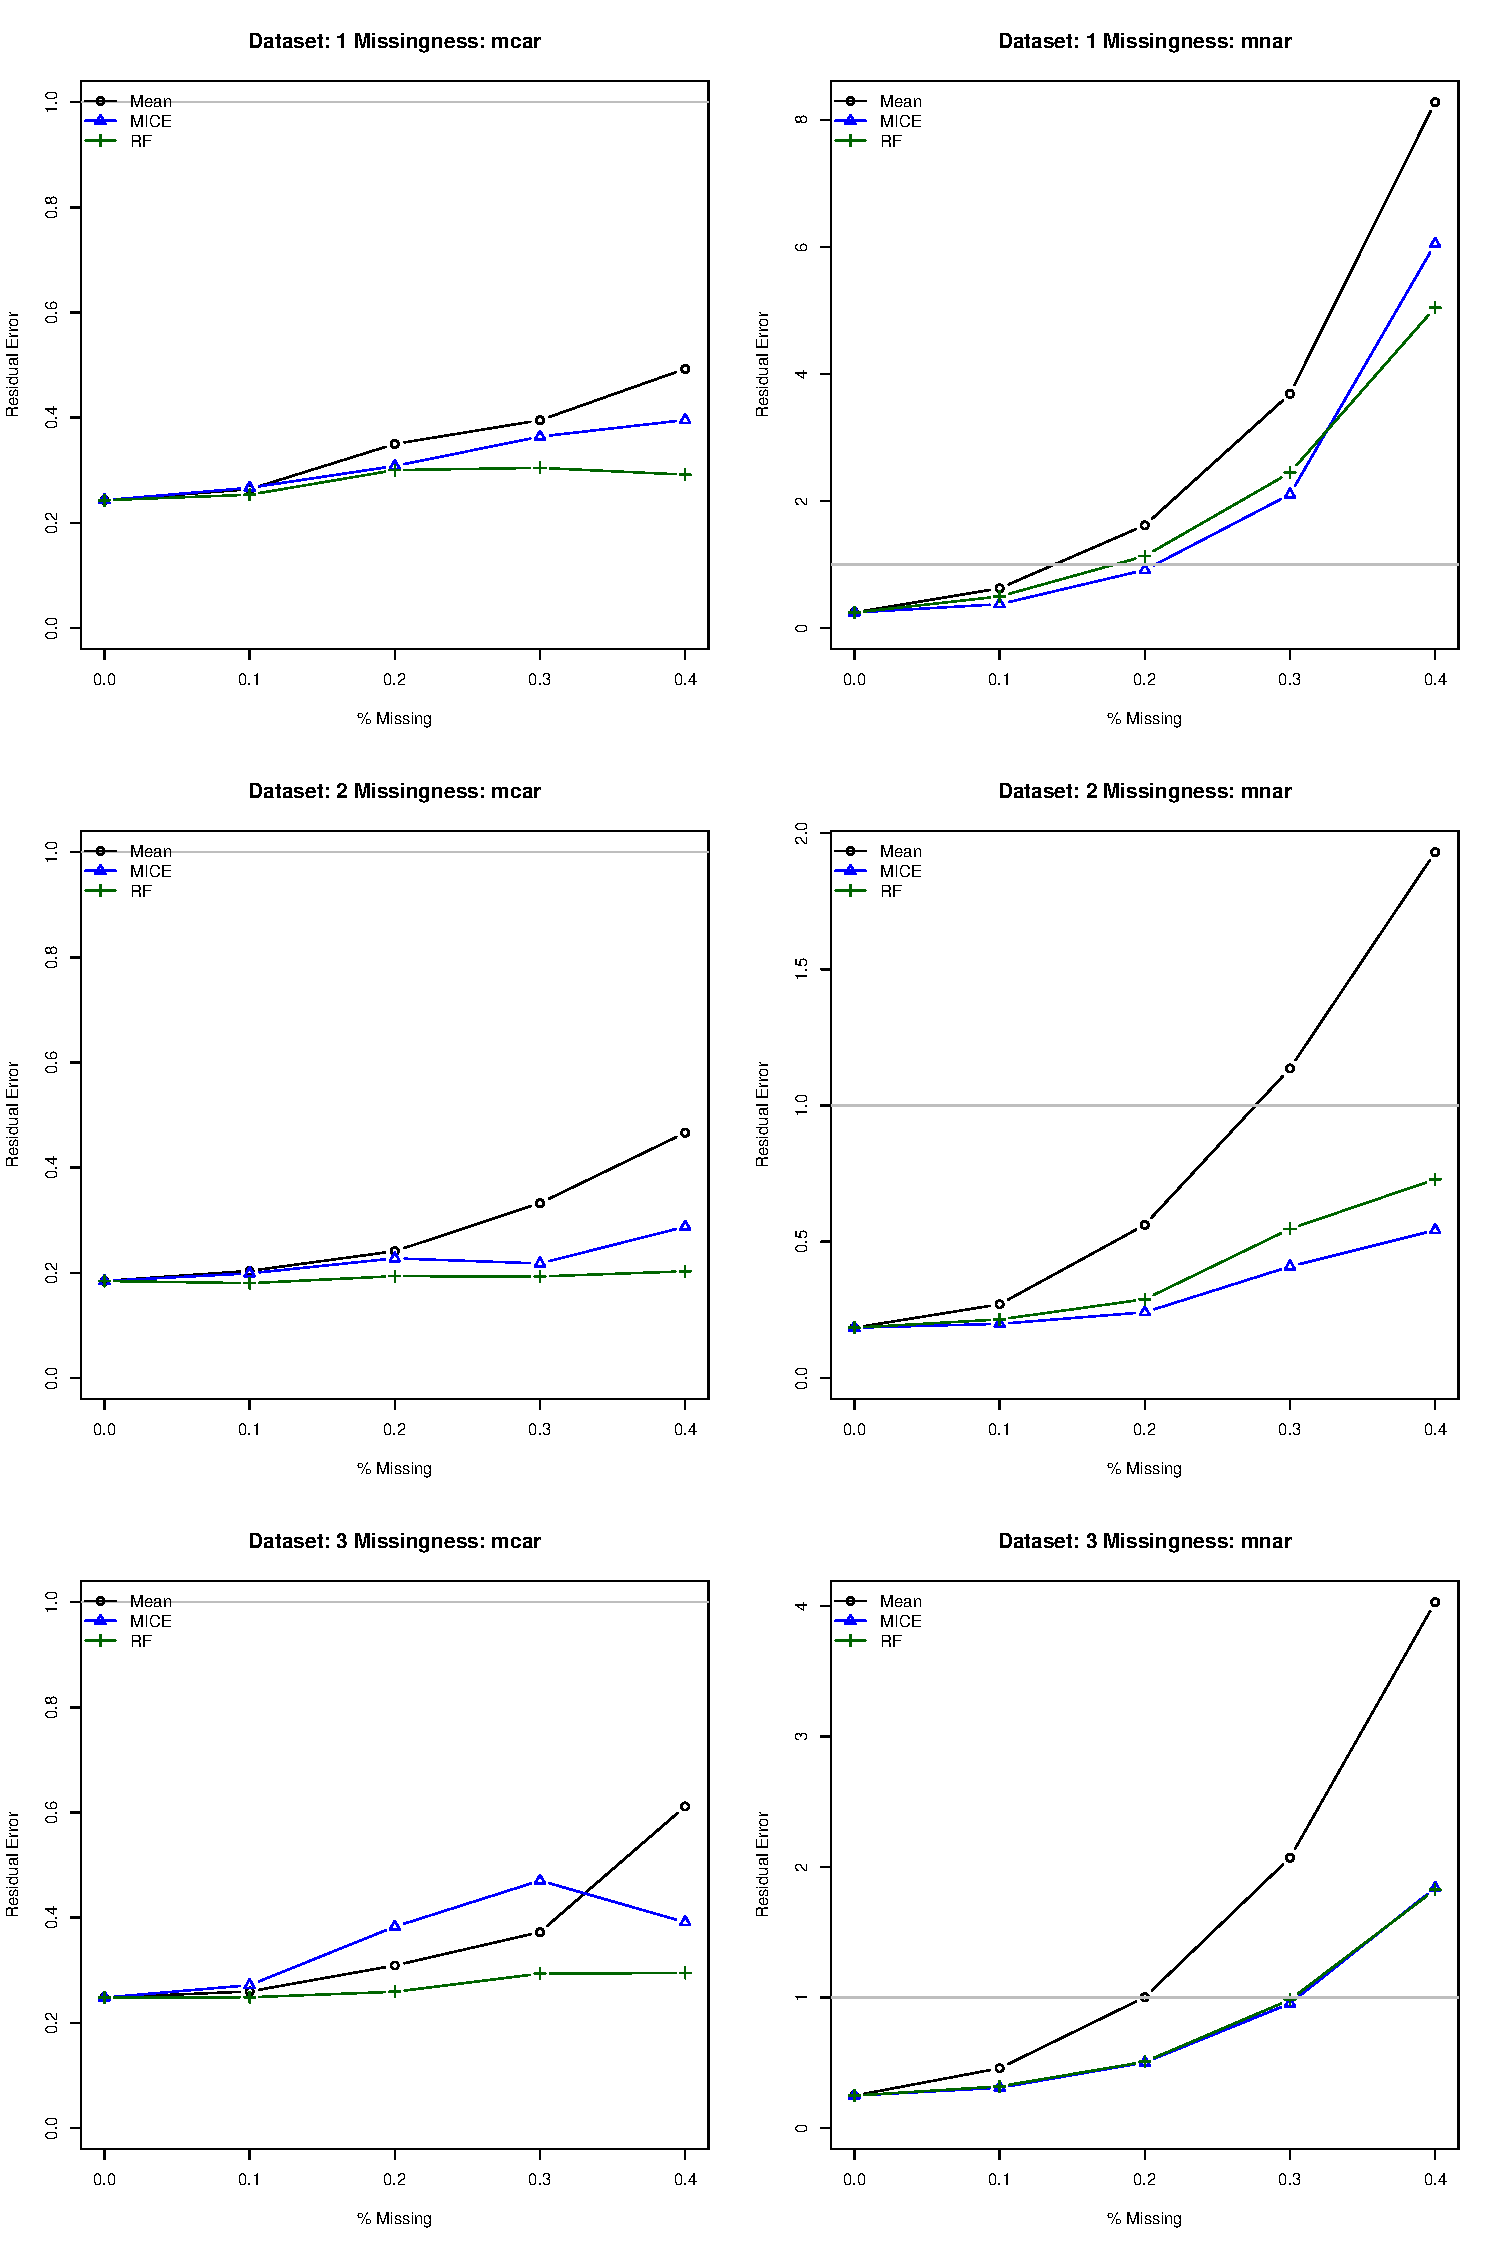
\includegraphics{error_plot_dataset.pdf}
\caption{Figure 1: Error}
\end{figure}


\end{document}
